\documentclass[10pt]{article}

\usepackage{fancyhdr}
\usepackage{extramarks}
\usepackage{amsmath}
\usepackage{amsthm}
\usepackage{amsfonts}
\usepackage{tikz}
\usepackage{ragged2e}
\usetikzlibrary{automata,positioning}
\usepackage{setspace}
\usepackage{etoolbox}
\usepackage{enumitem}
\usepackage{hyperref}
\hypersetup{colorlinks=true,allcolors=blue}
\usepackage{hypcap}
\usepackage{graphicx}    %for figure environment.
\usepackage{calc}
\usepackage{ifthen}
\usepackage{tikz}
\usepackage{longtable}
\usepackage{lipsum}
\usepackage{verbatim}
\usepackage{enumitem}
\setlist[enumerate]{itemsep=0mm}
\setlist[itemize]{itemsep=0mm}
\usepackage{pstricks-add}
\usepackage{pstricks}
\usepackage{rotating}
\usepackage[]{algorithm2e}
\usepackage{pdfpages}


\makeatletter
\pretocmd{\@sect}{\singlespacing}{}{}
\pretocmd{\@ssect}{\singlespacing}{}{}
\apptocmd{\@sect}{\singlespacing}{}{}
\apptocmd{\@ssect}{\singlespacing}{}{}
\makeatother

%
% Basic Document Settings
%
\newcommand{\ts}{\textsuperscript}

%\begin{comment}
\topmargin=-0.45in
\evensidemargin=0in
\oddsidemargin=0in
\textwidth=6.5in
\textheight=9.0in
\headsep=0.25in
%\end{comment}

\linespread{1.1}

\pagestyle{fancy}
\lhead{\hmwkAuthorName}
\chead{\textbf{\hmwkClass : \hmwkTitle}}
\rhead{\hmwkAuthorNumber}
\lfoot{\lastxmark}
\cfoot{\thepage}

\renewcommand\headrulewidth{0.4pt}
\renewcommand\footrulewidth{0.4pt}

\setlength\parindent{0pt}

%
% Create Problem Sections
%


\setcounter{secnumdepth}{0}
\newcounter{partCounter}
\newcounter{homeworkProblemCounter}
\setcounter{homeworkProblemCounter}{1}
\nobreak\extramarks{Problem \arabic{homeworkProblemCounter}}{}\nobreak{}

%
% Homework Problem Environment
%
% This environment takes an optional argument. When given, it will adjust the
% problem counter. This is useful for when the problems given for your
% assignment aren't sequential. See the last 3 problems of this template for an
% example.
%


%
% Homework Details
%   - Title
%   - Due date
%   - Class
%   - Section/Time
%   - Instructor
%   - Author
%

\newcommand{\hmwkTitle}{Assignment 3\ \ }
\newcommand{\hmwkDueDate}{Sunday, December 3\ts{rd}, 2017}
\newcommand{\hmwkClass}{CSC411}
\newcommand{\hmwkClassTime}{Section A}
\newcommand{\hmwkClassInstructor}{Steven Chuang}
\newcommand{\hmwkClassTeachingAssistant}{Natalia Mykhaylova}
\newcommand{\hmwkAuthorName}{Gokul K. Kaushik}
\newcommand{\hmwkAuthorNumber}{999878191}
\newcommand{\schoolmate}{\textsc{School-Mate }}

\newcommand\Tstrut{\rule{0pt}{2.6ex}}       % "top" strut
\newcommand\Bstrut{\rule[-0.9ex]{0pt}{0pt}} % "bottom" strut
\newcommand{\TBstrut}{\Tstrut\Bstrut} % top&bottom struts
%
% Title Page
%

\title{
    \vspace{2in}
    \textmd{\textbf{\hmwkClass:\ \hmwkTitle}}\\
    \vspace{0.1in}\small{Due\ on\ \hmwkDueDate}\\
    \vspace{3in}
    \vspace{0.1in}\large{Student Name: \textbf{\hmwkAuthorName} } \\
    \vspace{0.1in}\large{Student Number: \textbf{\hmwkAuthorNumber} } \\
}

%\author{\textbf{\hmwkAuthorName}}
%\textbf{\hmwkAuthorNumber\}
\date{}

\renewcommand{\part}[1]{\textbf{\large Part \Alph{partCounter}}\stepcounter{partCounter}\\}

%
% Various Helper Commands
%

% Useful for algorithms
\newcommand{\alg}[1]{\textsc{\bfseries \footnotesize #1}}

% For derivatives
\newcommand{\deriv}[1]{\frac{\mathrm{d}}{\mathrm{d}x} (#1)}

% For partial derivatives
\newcommand{\pderiv}[2]{\frac{\partial}{\partial #1} (#2)}

% Integral dx
\newcommand{\dx}{\mathrm{d}x}

% Alias for the Solution section header
\newcommand{\solution}{\textbf{\large Solution}}

% Probability commands: Expectation, Variance, Covariance, Bias
\newcommand{\E}{\mathrm{E}}
\newcommand{\Var}{\mathrm{Var}}
\newcommand{\Cov}{\mathrm{Cov}}
\newcommand{\Bias}{\mathrm{Bias}}
\renewcommand*\contentsname{Table of Contents}

\begin{document}
\maketitle
\pagebreak

\begin{center} \tableofcontents \end{center}
\pagebreak

\clearpage
\setcounter{page}{1}

\section{1 - 20 Newsgroup Predictions}

\subsection{3 methods chosen}

\textbf{I chose to use the \textit{tf-idf} feature representation.} I felt that logically it would give me a better result as it uses frequency. \textbf{All subsequent information is based using this feature set}.
\\ \\
The 3 models (other than the baseline model) that were chosen are: 
\begin{enumerate}
\item SGD
\item Logistic Regression
\item Random Forest
\end{enumerate}

\subsection{Train and Test Accuracies and Losses}

\begin{enumerate}
\item Baseline Model
	\begin{enumerate}
	\item Train accuracy: 59.8727
	\item Test accuracy: 45.7912
	\item Train loss: 0.4012
	\item Test loss: 0.5420
	\end{enumerate}

\item SGD
	\begin{enumerate}
	\item Train accuracy: 95.6248
	\item Test accuracy: 69.6096
	\item Train loss: 0.0437
	\item Test loss: 0.3039
	\end{enumerate}	

\item Logistic Regression
\begin{enumerate}
	\item Train accuracy: 89.5704
	\item Test accuracy: 67.7509
	\item Train loss: 0.1042
	\item Test loss: 0.3224
\end{enumerate}

\item Random Forest
\begin{enumerate}
	\item Train accuracy: 97.2777
	\item Test accuracy: 41.5825
	\item Train loss: 0.0272
	\item Test loss: 0.5841
\end{enumerate}
\end{enumerate}

\subsection{Picking the Best Hyper Parameters}
\begin{enumerate}
\item \textbf{SGD}: Hinge Loss was used as the loss function with an L2 penalization function. In order to get the best hyper parameters, the optimal regularized constant was determined through trial and error.

\item \textbf{Logistic Regression}: The hyper parameters were selected by a randomized search. The range of parameters were specified with a random state of 1 with no cross validation.

\item \textbf{Random Forest}: The default parameters were used. Increasing the randomness did not increase the training or test accuracy significantly. It was therefore assumed that the default parameters (provided by the library) was satisfiable.
\end{enumerate}



\subsection{Explain why you picked these 3 methods}
\begin{enumerate}
\item \textbf{SGD}: It has been known to work well with natural language processing problems (e.g. the given data set, where text needs to be classified). It was expected to perform better than the baseline model as there were many parameters that could be tuned to optimize performance. It worked as expected: it had the highest performance among models based on the test set accuracy of 69\%.

\item \textbf{Logistic Regression}: Logistic regression does not over fit for the data and the loss functions give it flexibility for penalization. Hence it seemed a good choice when correlated features are being used. The expectation was that it would work better than the base line model for the same settings (penalization, etc.) It works as expected as it did not assume independence among features given a class (the baseline predictor does).

\item \textbf{Random Forest}: Random forest models are good with complex classification tasks. The classification could involve taking advantage of the meaning behind text (natural language processing). It performed poorer than the baseline model. The Random forest had a high training accuracy which is expected (as it memorizes the data and has a tendency to over fit). However, this did not translate into test cases perhaps because the feature information was not continuous to provide for an obvious trend or perhaps due to the over fit.

\end{enumerate}

\pagebreak

\subsection{Best Classifier and Confusion Matrix}

The best classifier was the \textbf{SGD classifier} with a test accuracy of 69\% and a training accuracy of 95\%.
\\ \\
The class with the most confusion (i.e. which had the highest number of false predictions associated with it) was \textbf{talk.religion.misc (feature 19)}.
\\ \\
The two classes that the classifier were most confused about were \textbf{talk.politics.guns (feature 16)} and \textbf{talk.politics.misc (feature 18)}.
\\ \\
The confusion matrix is plotted below: 

\begin{center}
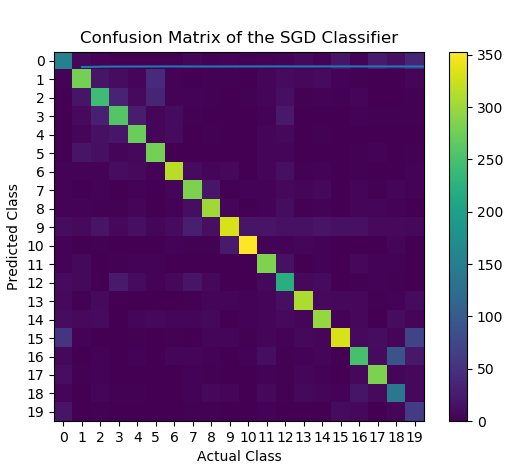
\includegraphics[scale=0.75]{1.png}
\end{center}




\section{2 - Training SVM with SGD}
\subsection{2.1 - SGD with Momentum}

Plotting $w_t$ for each time step $t$ by applying the iterative stochastic gradient-descent on $ f(w) = 0.01w^2$, we get the following graph (for $\beta = 0.1$ and $\beta = 0.9$ for upto 200 time-steps):

\begin{center}
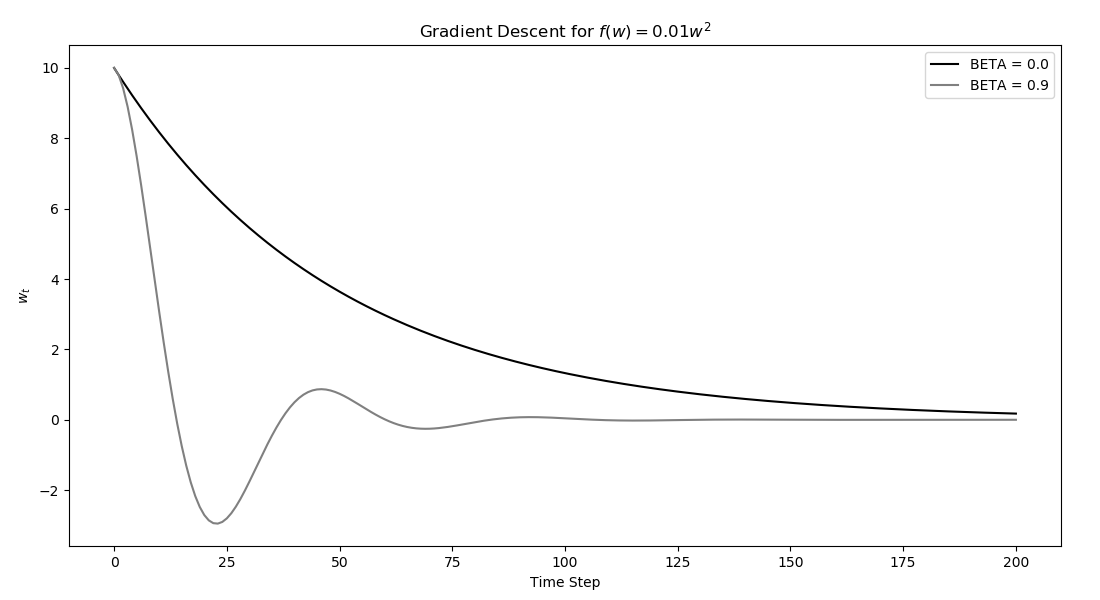
\includegraphics[scale=0.5]{2_1.png}
\end{center}



\subsection{2.2 -Training SVM}
\subsection{2.3 - Apply 4-vs-9 Digits on MNIST}

Two SVM models were trained using gradient descent. Both models had the following properties: 

\begin{enumerate}
\item A learning rate of $\alpha = 0.05 $
\item A penalty of $C = 1.0$
\item Mini-batch sizes of $m = 100$ and $T = 500$
\end{enumerate}

Model 1 and 2 had different $\beta$ values.

\begin{enumerate}
\item \textbf{Model 1}: $\beta = 0 $ 
\item \textbf{Model 2}: $\beta = 0.1 $
\end{enumerate}


 For the first model use   = 0 and for the second use   = 0.1. For both of the trained models report the following:

\subsubsection{2.3.1 - Training Loss}

\begin{enumerate}
\item \textbf{Model 1 ($\beta = 0 $) Training Loss}: 0.3829
\item \textbf{Model 2 ($\beta = 0.1 $) Training Loss}: 0.3743
\end{enumerate}

\subsubsection{2.3.2 - Test Loss}

\begin{enumerate}
\item \textbf{Model 1 ($\beta = 0 $) Test Loss}: 0.3748
\item \textbf{Model 2 ($\beta = 0.1 $) Test Loss}: 0.3672
\end{enumerate}

\subsubsection{2.3.3 - Classification Accuracy on the Training Set}

\begin{enumerate}
\item \textbf{Model 1 ($\beta = 0 $) Classification Accuracy on Training Set}: 0.9139
\item \textbf{Model 2 ($\beta = 0.1 $) Classification Accuracy on Training Set}: 0.9127
\end{enumerate}

\subsubsection{2.3.4 - Classification Accruacy on the Test Set}

\begin{enumerate}
\item \textbf{Model 1 ($\beta = 0 $) Classification Accuracy on Test Set}: 0.9154
\item \textbf{Model 2 ($\beta = 0.1 $) Classification Accuracy on Test Set}: 0.9125
\end{enumerate}


\subsubsection{2.3.5 - Plot \textbf{$w$} as a 28 $\times $ 28 image }

$\textbf{w}$ for Model 1 ($\beta = 0 $): 

\begin{center}
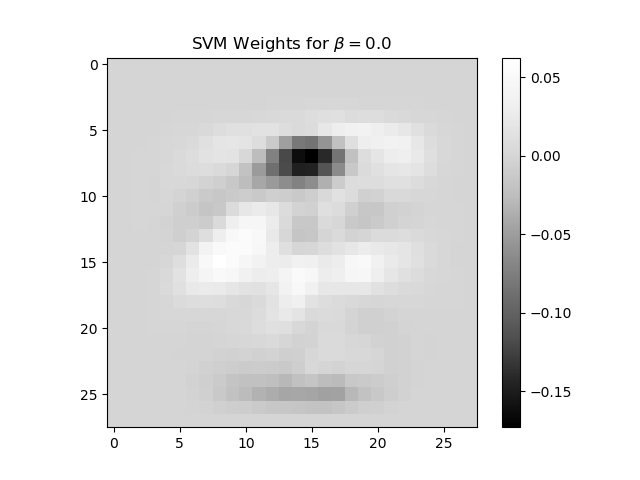
\includegraphics[scale=0.5]{2_3_1.png}
\end{center}

$\textbf{w}$ for Model 2 ($\beta = 0.1 $): 

\begin{center}
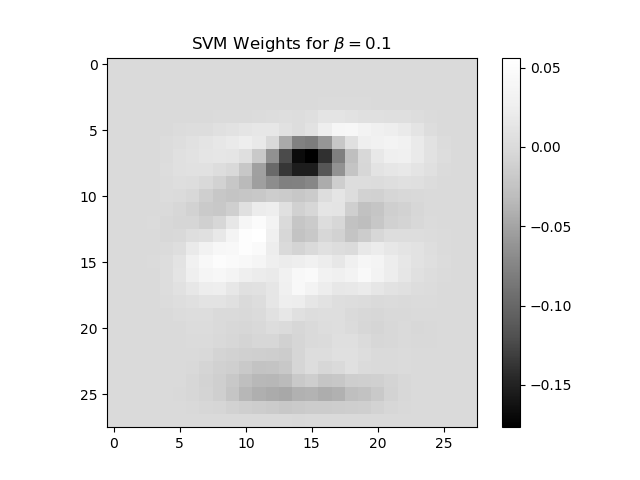
\includegraphics[scale=0.5]{2_3_2.png}
\end{center}


\section{3 - Kernels}
\subsection{3.1 - Positive Semi definite and Quadratic Form}

Prove that a symmetric matrix $K \in \mathbb{R}^{d \times d} $ is a positive semi definite iff for all vectors $x$ we have $\textbf{x}^{T}K\textbf{x} \geq 0$.
\\ \\
Proof: 

\[
K\textbf{x} = \lambda \textbf{x}
\]

where $\lambda$ is the eigenvalue and $\textbf{x}$ is the eigenvector. 
\\ \\
Suppose $\textbf{x}$ is an eigenvector of $K$ and replacing $K\textbf{v}$ with $\lambda \textbf{v}$ (from the definition of an eigenvector and eigenvalue above):
\[
\textbf{x}^{T}K\textbf{x} = \textbf{x}^{T} \textbf{x} \lambda
\]

\[
\textbf{x}^{T}K\textbf{x} = |\textbf{x}|^{2} \lambda
\]

Therefore, as $|\textbf{x}|^{2} \geq 0$, for the equation $\textbf{x}^{T}K\textbf{x} \geq 0$, the eigenvalue must be: $\lambda \geq 0$. Since it is a semi-definite matrix, where the eigenvalues $\geq 0$, this holds true.  


\subsection{3.2 - Kernel Properties}
\subsubsection{3.2.1 - Prove Property $k(\textbf{x},\textbf{y}) = \alpha $ is a kernel for $\alpha > 0$}

\[
\phi(\textbf{x}) = \sqrt{\alpha}
\]

\[
k(\textbf{x},\textbf{y}) = \langle \phi(\textbf{x}), \phi(\textbf{y}) \rangle
\]

\[
k(\textbf{x},\textbf{y}) = \sqrt{\alpha} \sqrt{\alpha}
\]

\[
k(\textbf{x},\textbf{y}) = \alpha
\]

\subsubsection{3.2.2 - Prove Property $k(\textbf{x},\textbf{y}) = f(\textbf{x}) \cdot f(\textbf{y}) $ is a kernel for $ f: \mathbb{R}^{d} \rightarrow \mathbb{R}$}

\[
\phi(\textbf{x}) = f(\textbf{x})
\]

\[
k(\textbf{x},\textbf{y}) = \langle \phi(\textbf{x}), \phi(\textbf{y}) \rangle
\]

\[
k(\textbf{x},\textbf{y}) = f(\textbf{x}) \cdot f(\textbf{y})
\]


\subsubsection{3.2.3 - Prove Property If $k_1(\textbf{x},\textbf{y})$ and $k_2(\textbf{x},\textbf{y})$ are kernels then $k(\textbf{x},\textbf{y}) = a \cdot k_1((\textbf{x},\textbf{y}) + b \cdot k_2((\textbf{x},\textbf{y})$ for $a,b > 0$ is a kernel}

Let $\textbf{K}_1$ and $\textbf{K}_2$ be gram matrices
\\ \\
Therefore: 

\[
\textbf{x}^{T} \textbf{K}_1 \textbf{x} \geq 0
\]

and 

\[
\textbf{x}^{T} \textbf{K}_2 \textbf{x} \geq 0
\]
 
Let: 

\[
\textbf{K}_{3}(\textbf{x},\textbf{y}) = a \textbf{K}_{1}(\textbf{x},\textbf{y}) + b  \textbf{K}_{2}(\textbf{x},\textbf{y})
\]

\[
\textbf{K}_{3} = a \textbf{K}_{1} + b  \textbf{K}_{2}
\]

\[
\textbf{x}^{T} \textbf{K}_3 \textbf{x} = \textbf{x}^{T} ( a \textbf{K}_{1} + b  \textbf{K}_{2}) \textbf{x}
\]

\[
\textbf{x}^{T} \textbf{K}_3 \textbf{x} = a \textbf{x}^{T} \textbf{K}_1 \textbf{x} + b \textbf{x}^{T} \textbf{K}_2 \textbf{x}
\]

and using 3.2.1's proof, $\textbf{K}_{3}(\textbf{x},\textbf{y})$ is a kernel, we get: 

\[
a \textbf{x}^{T} \textbf{K}_1 \textbf{x} + b \textbf{x}^{T} \textbf{K}_2 \textbf{x} \geq 0 \text{ for } a,b > 0
\]


\subsubsection{3.2.4 - Prove Property If $k_1(\textbf{x},\textbf{y})$ is a kernel then $k(\textbf{x},\textbf{y}) = \frac{k_1(\textbf{x},\textbf{y})}{\sqrt{k_1(\textbf{x},\textbf{x})} \sqrt{k_1(\textbf{y},\textbf{y})}}$ is a kernel}

Let:

\[
k_1(\textbf{x},\textbf{y}) = \langle \phi(\textbf{x}), \phi(\textbf{y}) \rangle
\]

\[
\langle \phi(\textbf{x}), \phi(\textbf{y}) \rangle = \phi (\textbf{x}) \cdot \phi (\textbf{y})
\]

In equation $k_1(\textbf{x},\textbf{y})$, replacing all the instances of $k_1(\textbf{x},\textbf{y})$ with $ \phi (\textbf{x}) \cdot \phi (\textbf{y})$: 


\[
k(\textbf{x},\textbf{y}) = \frac{k_1(\textbf{x},\textbf{y})}{\sqrt{k_1(\textbf{x},\textbf{x})} \sqrt{k_1(\textbf{y},\textbf{y})}}
\]

\[
k(\textbf{x},\textbf{y}) = \frac{\phi (\textbf{x}) \cdot \phi (\textbf{y})}{\sqrt{\phi (\textbf{x}) \cdot \phi (\textbf{x})} \sqrt{\phi (\textbf{y}) \cdot \phi (\textbf{y})}}
\]

\[
k(\textbf{x},\textbf{y}) = \frac{\phi (\textbf{x}) \cdot \phi (\textbf{y})}{|\phi (\textbf{x})| |\phi (\textbf{y})|}
\]

\[
k(\textbf{x},\textbf{y}) = \frac{k_1(\textbf{x},\textbf{y})} {|\phi (\textbf{x})| |\phi (\textbf{y})|}
\]

Let $\textbf{K}_1$ for matrix $k_1(\textbf{x},\textbf{y})$ be a gram matrix. Therefore: 

\[
\textbf{x}^{T} \textbf{K}_1 \textbf{x} \geq 0
\]

Multiplying each entry of $k_1$ will result in a positive value. Therefore, $k(\textbf{x},\textbf{y})$ is a kernel.


\pagebreak


\end{document}

$





